\documentclass{report}

\usepackage[utf8]{inputenc}
\usepackage[T1]{fontenc}
\usepackage[a4paper,left=75px,right=75px,top=75px,bottom=75px]{geometry}
\usepackage[francais,english]{babel}
\usepackage{graphicx}

\newcommand{\HRule}{\rule{\linewidth}{0.5mm}}
\newcommand{\blap}[1]{\vbox to 0pt{#1\vss}}
\newcommand\AtUpperLeftCorner[3]{%
  \put(\LenToUnit{#1},\LenToUnit{\dimexpr\paperheight-#2}){\blap{#3}}%
}
\newcommand\AtUpperRightCorner[3]{%
  \put(\LenToUnit{\dimexpr\paperwidth-#1},\LenToUnit{\dimexpr\paperheight-#2}){\blap{\llap{#3}}}%
}

\begin{document}

\begin{titlepage}

\enlargethispage{2cm}


 
\includegraphics[height=70]{./Schema/esme-logo.jpg}
% esme-logo.jpg: 0x0 pixel, 300dpi, 0.00x0.00 cm, bb=

\begin{center}
\vspace*{5cm}
\Huge\bf{Rapport de projet} \\ 
\vspace*{1.5cm}
\LARGE{Conception et r\'{e}alisation du dispositif de commande et de s\'{e}curit\'{e} d'un stimulateur \'{e}pidural transcutan\'{e}}

\end{center}

\vspace*{7cm}
\begin{center}
\Large{Narimane A\"{i}t Boudaoud \\Ursula de Vaux-Bidon \\Ma\"{e}va Galleron \\Europe Olympia Massenot \\}
\vspace*{1cm}
\Large{Projet encadr\'{e} par Monsieur Gilbert PRADEL}
\end{center}


\end{titlepage}

\chapter*{Remerciements}
\large
Nous tenions \`{a} remercier notre encadrant Monsieur Gilbert Pradel pour sa pr\'{e}sence constante et son aide dans l'avanc\'{e}e de ce projet. \\
Nous remercions \'{e}galement notre chef de d\'{e}partement Monsieur Christian Touseau gr\^{a}ce auquel nous b\'{e}n\'{e}ficions d’un bon environnement de travail et d’un mat\'{e}riel optimal. \\
Merci enfin \`{a} tous nos camarades de la 3D pour leur soutien moral durant le d\'{e}roulement du semestre. 

\newpage

\tableofcontents

\newpage


\chapter*{Intitul\'{e} du projet}
\begin{center}
\textbf{Conception et r\'{e}alisation du dispositif de commande et de s\'{e}curit\'{e} d'un stimulateur \'{e}pidural transcutan\'{e}}
\vspace*{1cm}
\end{center}
Ce projet est conduit par l'h\^{o}pital Raymond Poincar\'{e} \`{a} Garches et se fait avec la collaboration de l'ENS Cachan. Notre travail sera encadr\'{e} par Monsieur Gilbert Pradel.

\chapter*{Introduction}

Ce projet s’inscrit dans le cadre de notre derni\`{e}re ann\'{e}e \`{a} l’ESME Sudria et traite de la conception et de la r\'{e}alisation du 
dispositif de commande et de s'\'{e}curit\'{e} d'un stimulateur \'{e}pidural transcutan\'{e}. Ce dispositif s’adresse \`{a} des 
patients atteints de l\'{e}sions plus ou moins s\'{e}v\`{e}res de la moelle \'{e}pini\`{e}re et ayant perdu totalement ou en partie l’usage 
de la marche. En effet, il s’agit ici de stimuler \'{e}lectriquement un g\'{e}n\'{e}rateur spinal de marche permettant ainsi de
retrouver une mobilit\'{e} des membres inf\'{e}rieurs.\\\\
L’objectif est donc pour nous de pouvoir r\'{e}ceptionner des donn\'{e}es d’intensit\'{e} et de tension relatives au dispositif de stimulation et de faire en sorte que le m\'{e}decin en charge de l’exp\'{e}rience 
puisse acc\'{e}der \`{a} ces donn\'{e}es et ce, en association avec un syst\`{e}me permettant d’assurer la s\'{e}curit\'{e} du patient. \\ \\
Notre travail est conduit par l'h\^{o}pital Raymond Poincar\'{e} \`{a} Garches et se fait avec la collaboration de l'ENS Cachan.\\ \\
Notre \'{e}quipe est constitu\'{e}e de quatre membres ayant tous suivi le m\^{e}me cursus au sein de l’ESME Sudria et appartenant 
au laboratoire \'{e}lectronique et Syst\`{e}mes embarqu\'{e}s. Le projet est encadr\'{e} par Monsieur Gilbert PRADEL.

\chapter{Contexte}

\section{Etat de l'art}

Ce n'est qu'au d\'{e}but du XX\`{e}me si\`{e}cle (1911) que G.T. Brown [7], associ\'{e} \`{a} C. Sherrington,
apporta une d\'{e}monstration que la locomotion n'\'{e}tait pas li\'{e}e \`{a} un r\'{e}flexe secondaire \`{a} une
stimulation p\'{e}riph\'{e}rique (hypoth\`{e}se initialement \'{e}mise par Sherrington) mais \`{a} l'activation
d'un g\'{e}n\'{e}rateur spinal de marche (GSM) situ\'{e} dans la moelle lombaire.\\
L'organisation des fibres nerveuses arrivant \`{a} la moelle (aff\'{e}rences primaires), moto et interneurones de cette r\'{e}gion de la moelle lombaire a \'{e}t\'{e} bien pr\'{e}cis\'{e}e par des chercheurs
su\'{e}dois (A. Lundberg, E. Jankowska puis S. Grillner) dans les ann\'{e}es 1960-80. [8].\\
L'existence de ce GSM a \'{e}t\'{e} clairement d\'{e}montr\'{e}e chez tous les mammif\`{e}res sauf chez les
primates (singes, bip\`{e}des ou quadrup\`{e}des et hommes).\\ \\

Il existe cependant de nombreux arguments montrant que ce g\'{e}n\'{e}rateur spinal existe chez
l'homme. L'un des plus convaincants [9] est la possibilit\'{e}, chez des patients ayant une
section compl\`{e}te de la moelle \'{e}pini\`{e}re, de d\'{e}clencher une activit\'{e} locomotrice des muscles
des membres inf\'{e}rieurs par stimulation \'{e}lectrique des aff\'{e}rences nerveuses arrivant dans la
moelle au niveau L2 L3 (soit au niveau de la 11, 12\`{e}me vert\`{e}bre dorsale).\\
Des \'{e}lectrodes de stimulation reli\'{e}es \`{a} un boitier externe sont pos\'{e}es, chirurgicalement, sur
le tissu recouvrant la moelle et les racines post\'{e}rieures qui entrent dans la moelle au niveau
de la vert\`{e}bre D12 (tissu \'{e}pidural). Il a \'{e}t\'{e} d\'{e}montr\'{e} que ces stimulations (salves de 3 chocs
de 0,5ms pour une intensit\'{e} 8 \`{a} 10 mA et une fr\'{e}quence 30Hz) activent les aff\'{e}rents de gros
calibre (fibres Ia, Ib, et cutan\'{e}\'{e}es) qui dans la moelle se connectent aux diff\'{e}rents neurones
moteurs et aux interneurones de cette r\'{e}gion qui forment le g\'{e}n\'{e}rateur spinal de marche.\\ \\

Un premier travail [10] a \'{e}t\'{e} publi\'{e} en 2011 dans un grand journal de m\'{e}decine, le Lancet,
rapportant l'observation d'un homme de 23 ans incapable de mobiliser volontairement ses
membres inf\'{e}rieurs apr\`{e}s une l\'{e}sion importante de la moelle cervicale \`{a} la suite d'un
accident de la route. Grace \`{a} ces stimulations, et apr\`{e}s une r\'{e}\'{e}ducation 170 s\'{e}ances, (de 4
heures sur une dur\'{e}e de 26 mois) il lui est possible de marcher (pendant la stimulation).\\ \\

Depuis cette date plusieurs publications, dans de grands journaux (m\'{e}dicaux et
scientifiques), principalement de cette \'{e}quipe (Russo-Am\'{e}ricaine), ont rapport\'{e} quelques
cas semblables. Il semble donc scientifiquement d\'{e}montr\'{e} que, chez l'homme, une
stimulation \'{e}lectrique de fibres nerveuses est capable d'activer un g\'{e}n\'{e}rateur de marche
situ\'{e} dans la moelle lombaire.\\ \\

Par contre se pose toujours un probl\`{e}me m\'{e}dical : cette technique est-elle utile pour ce type
de patient ? Et, \'{e}ventuellement pour d'autres types de patients ayant des troubles de la
marche secondaires \`{a} une l\'{e}sion moins importante de la moelle ou du cerveau par exemple.D\'{e}montrer qu'il existe un g\'{e}n\'{e}rateur spinal de marche est certes important, mais d\'{e}montrer
que l'activation de ce g\'{e}n\'{e}rateur est fonctionnellement utile aux patients dans la vie de tous
les jours est diff\'{e}rent. \\

Plus r\'ecemment [11][12] a \'et\'e d\'ecrit une nouvelle possibilit\'e de stimuler le g\'en\'erateur spinal de 
locomotion 
chez l'homme en utilisant des stimulations \'electriques percutan\'ees et indolores et non dangereuses. En utilisant 
des courants  de faible dur\'ee et de forte intensit\'e. Cela a, m\'edicalement, une importance pratique massive en 
pratique m\'edicale. Il devient possible d'utiliser cette technique en pratique courante et montrer au patient (et aux 
soignants) si cette technique est efficace, ou non chez un patient donn\'e. 
De plus cette technique pourra \^etre utilis\'ee soit :
  
\begin{itemize}
    \item  chez des patients ayant une section, compl\`ete ou quasi compl\`ete, de la moelle, et dans ce cas, une 
implantation chirurgicale ult\'erieure du dispositif sera n\'ecessaire, mais le malade et les soignants seront tr\`es 
conscients de l'int\'er\^et, ou nom, de ce traitement,

    \item chez des patients c\'er\'ebro ou m\'edullo l\'es\'es (l\'esion incompl\`ete permettant la marche), ou 
des personnes \^ag\'es perdant l'automatisme de marche, la stimulation sera appliqu\'ee pendant la s\'eance de 
r\'e\'education de la locomotion, le patient et le soignant pourront juger de l'int\'er\^et (ou non) de cette 
technique. Le nombre de patients de ce type est consid\'erablement plus \'elev\'e que ceux ayant une section compl\`ete 
de la moelle.

\end{itemize}


 
\section{Cahier des charges }

Le projet comprend deux parties distinctes : \\

\begin{itemize}
    \item \textbf{L'ensemble haute tension} : A partir de batteries (et non du secteur pour d'\'{e}videntes
raisons de s\'{e}curit\'{e}́ ) une haute tension est g\'{e} n \'{e} r \'{e} e par un convertisseur \'{e} l \'{e} vateur de
type yback. Cet \'{e}l\'{e}vateur utilise un hacheur \`{a} haute fr\'{e} quence (300MHz environ) et
un transformateur \'{e} l \'{e} vateur pour arriver \`{a} une tension secondaire de l'ordre de
500V. L'intensit\'{e} inject\'{e} e dans le GSM est une salve de 10 impulsions de 33\mu s et de
500 mA maximum d'amplitude. Cette partie rel\`{e}ve de l'ENS de Cachan.
    
    \item \textbf{L'ensemble de contr\^ole-commande} qui doit :
   
    \begin{itemize}
        \item contr\^oler les grandeurs \'electriques (tensions et courants au primaire et au secondaire) au moyen de 
capteurs isol\'es,
        \item enregistrer ces grandeurs durant l'exp\'erimentation qui peut durer plusieurs dizaines de minutes,
        \item v\'erifier que les grandeurs ne d\'epassent pas des valeurs pr\'e\'etablies par le m\'edecin,
        \item concevoir une interface permettant au m\'{e}decin de contrôler le processus de traitement du patient
        \item v\'erifier que le syst\`eme est en \'etat d'assurer le bon d\'eroulement de l'exp\'erience.
    \end{itemize}
\end{itemize}

Notre objectif est donc d'\'{e}tudier, de choisir et de concevoir l'architecture du syst\`{e}me qui
permet le contrôle du processus de stimulation \'{e}pidurale et de le r\'{e}aliser.\\
Ce syst\`{e}me devant s'appliquer \`{a} des patients, la contrainte de s\'{e}curit\'{e} est tr\`{e}s importante.
Nous en avons d\'{e}j\`{a} fait r\'{e}f\'{e}rence dans la partie pr\'{e}c\'{e}dente.
    
\section{M\'{e}thode utilis\'{e}e}

Notre projet n’implique aucune chirurgie puisque les \'{e}lectrodes seront directement en
contact avec la peau : c’est le principe de la \textbf{stimulation transcutan\'{e}e}. Les structures
nerveuses choisies sont stimul\'{e}es par le biais d'\'{e}lectrodes fix\'{e}es directement sur la peau. Il
s'agit donc d’une m\'{e}thode non invasive qui permettrait aux patients paralys\'{e}s de pouvoir
retrouver une fonction motrice sans passer par la chirurgie. \\

\begin{center}
 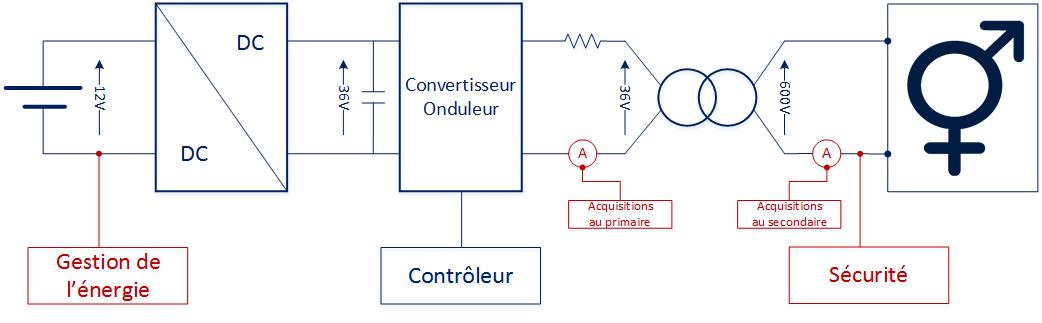
\includegraphics[height=90]{./Schema/sch_proj_modifie.jpg}
 % sch_proj_modifie.jpg: 0x0 pixel, 300dpi, 0.00x0.00 cm, bb=
\end{center}

L’objectif est d’injecter, via les \'{e}lectrodes, des impulsions d’intensit\'{e} tr\`{e}s importante sur un
temps tr\`{e}s court selon le mod\`{e}le suivant : \\



\section{Planification du projet}

Voici la planification de notre projet \`{a} l’aide d’un diagramme de GANTT gr\^{a}ce au logiciel
Microsoft Project 2016.\\
Dans le tableau est repr\'{e}sent\'{e} l’ensemble des t\^{a}ches que nous pr\'{e}voyons de r\'{e}aliser dans le
temps imparti du d\'{e}but au rendu final du projet.\\ \\
Dur\'{e}e du projet : \\
Date de d\'{e}but : lundi 3 octobre 2016 \\
Date de rendu : lundi 20 mars 2017

\section{Comparaison des cartes}

Afin de mettre en avant les avantages et inconv\'{e}nients des diff\'{e}rentes cartes susceptibles de
correspondre au projet, nous avons repr\'{e}sent\'{e} leurs caract\'{e}ristiques sous forme de tableau. \\
 

\begin{tabular}{|c|c|}
\hline
\multirow{BeagleBone Black}
& Nombre d’entr\'{e}es analogiques : 7 AIN (1,8V max) \\ 
& Temps de la conversion : 125 ns\\ 
& Pr\'{e}cision de la conversion : 12 bits \\ 
& Bluetooth : non \\ 
& Consommation : 460mA @5V \\ 
& I2C/SPI : oui/oui \\ \hline
\multirow{BeagleBone Black Wireless} 
& Nombre d’entr\'{e}es analogiques : 7 AIN  \\ 
& Temps de la conversion : 125 ns\\ 
& Pr\'{e}cision de la conversion : 12 bits \\ 
& Bluetooth : oui(4.1) \\ 
& Consommation :  \\ 
& I2C/SPI : oui/oui \\ \hline
\multirow{UDoo NEO} 
& Nombre d’entr\'{e}es analogiques : 6 AIN  \\ 
& Temps de la conversion : \\ 
& Pr\'{e}cision de la conversion : 12 bits \\ 
& Bluetooth : oui \\ & Consommation :  \\ 
& I2C/SPI : oui/oui \\ \hline
\multirow{Raspberry PI} 
& Nombre d’entr\'{e}es analogiques : non  \\ 
& Temps de la conversion : -\\ 
& Pr\'{e}cision de la conversion : - \\ 
& Bluetooth : non \\ 
& Consommation :  \\ 
& I2C/SPI : oui/oui \\ \hline
\multirow{Nordic SC nRF52832} 
& Nombre d’entr\'{e}es analogiques : 8 AIN  \\ 
& Temps de la conversion : de 3 \`{a} 40 us\\ 
& Pr\'{e}cision de la conversion : 12 bits \\ 
& Bluetooth : oui(BLE) \\ 
& Consommation : 5,5 \`{a} 7,5 uA @ 3,0V\\ 
& I2C/SPI : oui/oui \\ \hline
\multirow{Texas Instrument CC2540} 
& Nombre d’entr\'{e}es analogiques : 9 AD0 (VDD +0,3 V)  \\ 
& Temps de la conversion : de 2,1 us \`{a} 27 us\\ 
& Pr\'{e}cision de la conversion : 16 bits \\ 
& Bluetooth : non \\ 
& Consommation : 6,5 mA @ 3.0V \\ 
& I2C/SPI : oui/oui \\ \hline
\multirow{Freescale MKL25Z} 
& Nombre d’entr\'{e}es analogiques : 9 AD0 (VDD +0,3 V)  \\ 
& Temps de la conversion : de 2,1 us \`{a} 27 us\\ 
& Pr\'{e}cision de la conversion : 16 bits \\ 
& Bluetooth : non \\ 
& Consommation : 6,5 mA @ 3.0V \\ 
& I2C/SPI : oui/oui \\ \hline
\multirow{Microchip PIC16F1619} 
& Nombre d’entr\'{e}es analogiques : 12 ANSEL  \\ 
& Temps de la conversion : 125 ns\\ 
& Pr\'{e}cision de la conversion : 10 bits \\ 
& Bluetooth : non \\ 
& Consommation : 32 ua/MHz @1,8V (XLP) \\ 
& I2C/SPI : oui/oui \\ \hline
\end{tabular}
 
\chapter{Conception du syst\`{e}me}

Nous pouvons diviser notre syst\`{e}me en plusieurs sous-parties :
\begin{itemize}
\item une partie de contrôle de l’intensit\'{e} au primaire et au secondaire qui nous permettra d’agir en fonction de sa valeur
\item une partie de contrôle de la tension au primaire et au secondaire qui nous permettra d’agir en cons\'{e}quence en fonction de la valeur
\item une partie gestion de la batterie
\item une partie acquisition des param\`{e}tres m\'{e}decins et transmission des informations
\end{itemize}

\begin{center}
 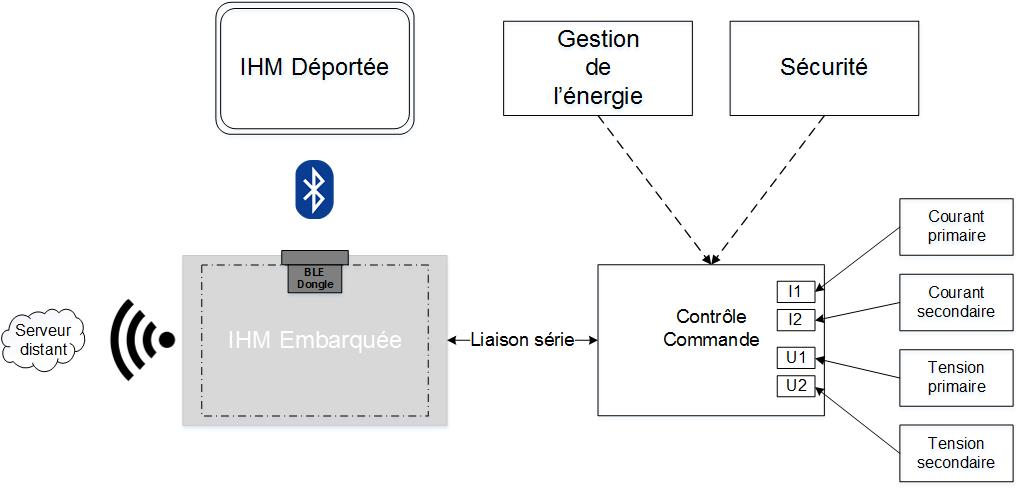
\includegraphics[height=150]{./Schema/sch_arch_sys_2.jpg}
 % sch_arch_sys_2.jpg: 0x0 pixel, 300dpi, 0.00x0.00 cm, bb=
\end{center}


\section{Cartes}

Parmi les cartes cit\'{e}es dans le tableau ci-dessus, nous avons choisi la BeagleBone Black. \\



Il s’agit d’une carte de d\'{e}veloppement de processeur ARM Cortex A8 32 bits, compatible
avec plusieurs syst\`{e}mes d’exploitation : Debian, Android etc.\\
Nous pouvons la connecter via USB host, Ethernet etc.\\
Elle est dot\'{e}e de 7 pins analogiques avec un temps de conversion de 125ns, d’un bus SPI et
I2C.\\
Elle ne consomme pas beaucoup et sa prise en main est simple.



En effet, il est possible d’y installer la sous-couche temps r\'{e}el manquante \`{a} Linux, dans notre
cas Xenomai, ce qui est un \'{e}l\'{e}ment essentiel dans l’acquisition des donn\'{e}es.\\
De plus, ceci nous permet de mettre en application les notions vues en cours de \textit{“Pilotes de
p\'{e}riph\'{e}riques pour OS embarqu\'{e}s}”.\\ \\

Ayant \'{e}t\'{e} amen\'{e}es \`{a} travailler \`{a} plusieurs reprises sur cette carte de d\'{e}veloppement, nous
sommes devenues famili\`{e}res avec celle-ci. Les outils d\'{e}j\`{a} disponibles dans la BeagleBone
Black permettent un gain de temps consid\'{e}rable. La BeagleBone Black va \^{e}tre utilis\'{e}e afin
d'acqu\'{e}rir des donn\'{e}es depuis les capteurs. Elles sont transmises par liaison Bluetooth vers
une Interface Homme Machine d\'{e}port\'{e}e.\\ \\

Pour l’acquisition des donn\'{e}es, 4 ports analogiques suppl\'{e}mentaires sont n\'{e}cessaires. Il est
donc impossible de g\'{e}rer l’\'{e}cran 4DSystems et l’acquisition sur la m\^{e}me carte BeagleBone
Black car cette derni\`{e}re ne poss\`{e}de que 7 ports analogiques. Il faut donc s\'{e}parer la gestion
des deux actions : une carte pour l’acquisition et une carte pour la gestion de l’\'{e}cran.\\
Pour un \'{e}change rapide d’informations entre les deux cartes, nous mettrons en place une
liaison s\'{e}rie.\\ \\

Pour \'{e}changer des informations avec l’interface Homme-Machine d\'{e}barqu\'{e}e nous
utiliserons une liaison Bluetooth.\\
Pour transmettre les donn\'{e}es de chaque manipulation vers un serveur ext\'{e}rieur, une liaison
wi-fi pourra \^{e}tre envisag\'{e}e.\\
De plus, pour un traitement de l’acquisition des donn\'{e}es simplifi\'{e}, nous avons d\'{e}cid\'{e} que la
carte g\'{e}rant l’\'{e}cran 4DSystem g\'{e}rera \'{e}galement la liaison Bluetooth.\\ \\

Par cons\'{e}quent, une modification de l’architecture de notre syst\`{e}me s’impose.
En effet, l’acquisition des donn\'{e}es se fera par une BeagleBone Black.\\
La gestion de l’\'{e}cran et de la liaison Bluetooth peut se faire par une BeagleBone Black
Wireless.\\
Cependant, pour des raisons techniques et financi\`{e}res, nous utiliserons pour la suite des
manipulations deux BeagleBone Black ainsi qu’un dongle Bluetooth (cl\'{e} bluetooth 4.0 BLE
CSR 8510).\\


\section{IHM embarqu\'{e}e}

Une Interface Homme-Machine doit \^{e}tre mise en place pour l’affichage du signal en temps
r\'{e}el. Pour cela, nous utilisons un \'{e}cran 4DSystems.



Nous souhaitons installer sur le syst\`{e}me \`{a} d\'{e}velopper un \'{e}cran qui diffusera l’\'{e}tat du signal
en temps r\'{e}el.\\
Notre int\'{e}r\^{e}t s’est pos\'{e} sur un \'{e}cran de la marque 4D Systems qui ne n\'{e}cessite que 4 ports
analogiques.\\
L’entreprise 4D Systems d\'{e}veloppe des modules afficheur pour des cartes \'{e}lectroniques,
telles que la BeagleBone Black, la Raspberry Pi, l’Arduino.\\
Nous avons choisi un module \'{e}cran tactile de 4.3’’ ADCAPE-43T, compatible avec la
BeagleBone Black.\\ \\

Sur une carte SD, nous avons charg\'{e} un environnement Xfce, que nous avons ensuite flash\'{e}
sur la BeagleBone Black.\\
Xfce est un environnement de bureau bas\'{e} sur la boîte \`{a} outils GTK+ qui se veut l\'{e}ger et
simple mais aussi complet, souple, modulaire et portable. Il est destin\'{e} aux syst\`{e}mes
d'exploitation apparent\'{e}s \`{a} UNIX.\\
Gr\^{a}ce \`{a} cela, nous avons pu obtenir un environnement Linux sur notre \'{e}cran qui nous
permettra ensuite de pouvoir observer le signal d\'{e}sir\'{e}.

\section{Gestion de l'intensit\'{e}}

Comme dit pr\'{e}c\'{e}demment, l’une des parties de notre projet consiste \`{a} acqu\'{e}rir les valeurs
de l’intensit\'{e} au primaire et au secondaire afin de pouvoir les comparer \`{a} des valeurs de
r\'{e}f\'{e}rence.\\

\begin{center}
 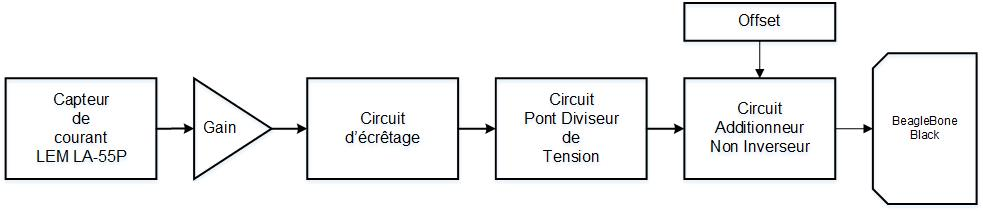
\includegraphics[height=80]{./Schema/sch_bloc_amp.jpg}
 % sch_bloc_amp.jpg: 0x0 pixel, 300dpi, 0.00x0.00 cm, bb=
\end{center}

Afin de pouvoir comparer la valeur de l’intensit\'{e} obtenue \`{a} la valeur de r\'{e}f\'{e}rence, nous
utilisons le convertisseur analogique-num\'{e}rique de la BeagleBone Black. Par cons\'{e}quent, la
tension de sortie de notre circuit doit \^{e}tre inf\'{e}rieure \`{a} 1,8V (tension maximale support\'{e}e par
la BBB sur une broche analogique). Pour \^{e}tre certaines de ne pas donner \`{a} la BeagleBone
Black une tension trop importante, nous nous sommes fix\'{e}es une valeur de 1,5V comme
tension de sortie maximale.\\ \\

Pour isoler l’intensit\'{e}, nous avons utilis\'{e} un capteur LEM LA 55-P.
Le LEM LA 55-P est un capteur de courant poss\'{e}dant une isolation galvanique entre le circuit
primaire (high power) et le circuit secondaire (circuit \'{e}lectrique).
Ce composant poss\`{e}de une r\'{e}sistance de mesure R M ajustable selon la valeur de la
temp\'{e}rature, de l’alimentation et la valeur maximale du courant. Dans notre cas, pour une
alimentation de \pm 12V, avec une valeur de courant maximale \`{a} \pm 50A, il nous faut :
R M = 100\Omega.



Pour obtenir une image exploitable, nous d\'{e}cidons de faire 10 tours de fil autour du capteur
afin de multiplier par 10 la valeur de courant mesur\'{e}e.\\
Ainsi nous obtenons : 10 tours x 50 mA = 500 mA.\\
Cependant, l’image n’\'{e}tant toujours pas assez \'{e}lev\'{e}e pour pouvoir l’exploiter, nous utilisons
un gain afin de r\'{e}soudre ce probl\`{e}me.\\
C’est dans cet objectif que nous nous sommes int\'{e}ress\'{e}es au composant INA114 qui est un
amplificateur polyvalent offrant une bonne pr\'{e}cision.\\
Une simple r\'{e}sistance externe R G permet de r\'{e}gler le gain de 1 \`{a} 10 000. Une protection
interne permet une r\'{e}sistance jusqu’\`{a} \pm 40 V sans aucun dommage.\\
Il fonctionne avec une alimentation allant jusqu’\`{a} minimum \pm 2.25V, permettant son
utilisation dans des syst\`{e}mes aliment\'{e} par des tensions de 5V. Sa consommation au repos
est de maximum 3mA. Ces 8 broches sont impl\'{e}ment\'{e}es comme ci-dessous :\\ 

\begin{tabular}{|c|c|}
\hline 
\multirow{1}
& R_{G} \hline
\multirow{2}
& V_{IN}- \hline
\multirow{3}
& V_{IN}+ \hline
\multirow{4}
& V- \hline
\multirow{5}
& Ref \hline
\multirow{6}
& V_{0} \hline
\multirow{7}
& V+ \hline
\multirow{8}
& RG \hline
\end{tabular} 

La documentation de l’INA114 nous indique la relation entre le gain et la r\'{e}sistance R_{G} : \\
\text{G = 1 +}\frac{50k\Omega}{R_{G}} \\
De plus, nous avons d\'{e}termin\'{e} une valeur de gain \'{e}gale \`{a} 160.\\
Ainsi, on aura :\\
\text{G = 1 +}\frac{50k\Omega}{R_{G}}\text{= 160}
\Leftrightarrow R_{G}\text{=314 \Omega} \\
Pour des raisons de budget, nous avons par la suite opt\'{e} pour le composant INA188 ayant
les m\^{e}mes caract\'{e}ristiques que le INA114.\\ \\

Par la suite, un circuit d'\'{e}cr\^{e}tage est mis en place pour limiter la tension entre +8V et -8V \`{a}
l’aide de deux diodes Zener. En effet, en mettant en place ces deux diodes en sens inverse,
l’addition des deux tensions respectives permet de limiter la tension, en positif et en n\'{e}gatif.

\begin{center}
 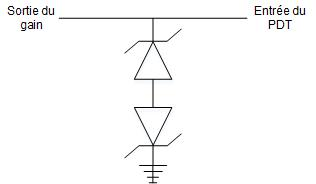
\includegraphics[height=90]{./Schema/ecretage.jpg}
 % ecretage.jpg: 0x0 pixel, 300dpi, 0.00x0.00 cm, bb=
\end{center}

L’utilisation de ponts diviseurs de tension nous permet de diminuer la tension en dessous du
seuil maximal de la BeagleBone.\\

\begin{center}
 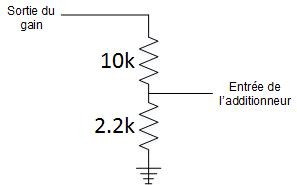
\includegraphics[height=110]{./Schema/div_tension.jpg}
 % div_tension.jpg: 0x0 pixel, 300dpi, 0.00x0.00 cm, bb=
\end{center}

Enfin, un additionneur permet de redresser cette tension entre +1,5V et -1,5V. \\

\begin{center}
 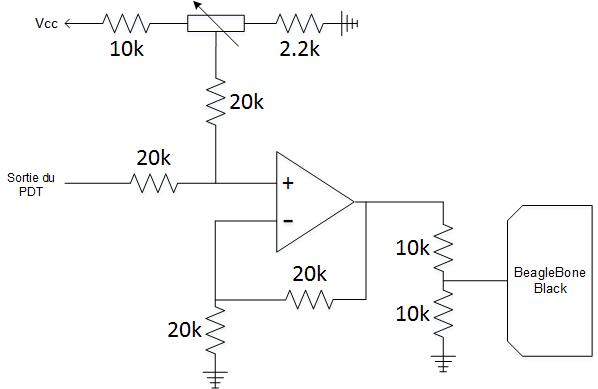
\includegraphics[height=150]{./Schema/add_offset.jpg}
 % add_offset.jpg: 0x0 pixel, 300dpi, 0.00x0.00 cm, bb=
\end{center}

Ce circuit nous permet donc de r\'{e}cup\'{e}rer l’intensit\'{e} de notre dispositif afin de pouvoir par la
suite la comparer au courant de r\'{e}f\'{e}rence.

\section{Gestion de la tension}

Le contrôle de la tension se basera sur le m\^{e}me principe que le contrôle de l’intensit\'{e}. Un
capteur va nous permettre d’isoler la tension et ainsi pouvoir traiter l’information en
fonction de sa valeur.\\



Le ADuM3190 est un amplificateur \`{a} erreur isol\'{e}, il est id\'{e}al pour les alimentations \`{a}
r\'{e}troaction. Il permet une meilleure r\'{e}ponse transitoire et contrairement aux solutions
optocoupleuses, qui ont un rapport de transfert de courant incertain d’un point de vue
dur\'{e}e de vie et \`{a} des temp\'{e}ratures \'{e}lev\'{e}es, la fonction de transfert ADuM3190 ne change
pas pendant toute sa dur\'{e}e de vie et est stable sur une large plage de temp\'{e}rature de -40 \degree C
\`{a} +125 \degree C.\\
L'ADuM3190 est emball\'{e} dans un petit paquet QSOP \`{a} 16 fils pour une tension nominale de
tension d'isolation de 2,5 kV.

\section{Acquisition des param\`{e}tres et transmission des information}

Afin de pouvoir g\'{e}rer l’acquisition des donn\'{e}es en temps r\'{e}el sur la BeagleBone Black, nous
avons d\'{e}cid\'{e} d’installer une sous couche temps r\'{e}el dure, RTLinux ou Xenomai. En effet on
souhaite que les limites temporelles donn\'{e}es au syst\`{e}me soient respect\'{e}es, m\^{e}me dans la
pire des situations d’ex\'{e}cution possible. Notre choix s’est port\'{e} sur Xenomai, car RTLinux ne
divulgue plus ses codes sources, et la license coûte ch\`{e}re.\\
Une acquisition en temps r\'{e}el sous Linux, permet :
\begin{itemize}
 \item d’envoyer des ordres au contrôleur
 \item de rendre l’OS de la carte non prioritaire
\end{itemize}

Cette sous-couche permettra de prendre en compte les interruptions g\'{e}n\'{e}r\'{e}es, entre
autres, lorsque l’on sera dans une situation dangereuse pour le patient.\\ \\

Lorsque l’on r\'{e}cup\`{e}re les donn\'{e}es acquises avec la deuxi\`{e}me BeagleBone, on souhaite les
envoyer \`{a} la tablette via une liaison Bluetooth, et \`{a} un serveur distant via une
communication Wi-Fi. \\ \\

Pour r\'{e}pondre \`{a} ces contraintes, nous avons choisi une BeagleBone Black Wireless. Celle-ci
poss\`{e}de \`{a} la fois un Bluetooth 4.1 BLE, et un module Wi-Fi, qui nous permettra d’envoyer les
donn\'{e}es de chaque patient \`{a} un serveur distant apr\`{e}s chaque manipulation du m\'{e}decin. \\ \\

Cependant, pour des raisons techniques et financi\`{e}res, deux BeagleBone Black seront
utilis\'{e}es pour la suite des manipulations. On ajoutera un dongle Bluetooth 4.0 de type BLE,
CSR 8510, pour effectuer les transferts de donn\'{e}es \`{a} la tablette. \\ \\

Le Bluetooth Low Energy r\'{e}duit fortement la consommation de la puce Bluetooth. Sa port\'{e}e
se compte en quelques dizaines de m\`{e}tres.\\ \\

Le serveur distant sera mis en place lorsque tout le syst\`{e}me aura \'{e}t\'{e} conçu.
Une modification de l’architecture de notre syst\`{e}me est donc n\'{e}cessaire.\\ \\

Suite \`{a} un TP effectu\'{e} en cours d’Android pour lequel nous avons dû configurer le Bluetooth.
Nous avons d\'{e}cid\'{e} d’utiliser cette m\^{e}me carte, Microchip Curiosity pour effectuer les tests
de configuration du Bluetooth. En effet celle-ci poss\`{e}de \'{e}galement un Bluetooth de type
BLE.


\section{Gestion de l'\'{e}nergie}

La gestion de la batterie est primordiale pour deux points : \\
Tout d’abord il faut s’assurer qu’un indicateur signalera la faible tension de celle-ci et donc
un chargement n\'{e}cessaire, ainsi que son processus de chargement.\\
La gestion de la batterie permettra \'{e}galement de s’assurer que la batterie a un niveau de
charge suffisant pour effectuer la s\'{e}quence introduite par les param\`{e}tres m\'{e}decins.\\ \\

Cependant, cette partie de notre syst\`{e}me de contrôle ne peut \^{e}tre effectu\'{e}e qu’une fois la
partie Transformateur du projet de l’ENS Cachan achev\'{e}e.

\chapter{Bilan de r\'{e}alisation \`{a} mi-projet}

\section{Etat des travaux}

Au cours de ce premier semestre, plusieurs t\^{a}ches ont \'{e}t\'{e} effectu\'{e}es : \\
\begin{itemize}
 \item Premi\`{e}res r\'{e}flexions sur le sujet, \'{e}tablissement des sch\'{e}mas de c\^{a}blages, calculs des
diff\'{e}rentes valeurs des composants des circuits (intensit\'{e}),
\item Veille concurrentielle, \'{e}tat de l’art dans le domaine de la stimulation \'{e}pidurale,
\item Analyse des diff\'{e}rentes cartes (BeagleBone, UDoo, Raspberry Pi, Nordic SC, Texas
Instrument, Freescale, Microchip, Arduino, Chip),
\item Test installation d’une sous-couche temps r\'{e}el sur BBB,
\item R\'{e}alisation de sch\'{e}mas sous EAGLE,
\item Mise en place du dongle Bluetooth.
\end{itemize}

\section{Difficult\'{e}s rencontr\'{e}es}

Tout au long de ce semestre, nous avons rencontr\'{e} un certain nombre de difficult\'{e}s.\\ \\

Nous avons choisi de travailler sur BeagleBone Black. Or, cette derni\`{e}re ne pr\'{e}sente pas
assez de broches analogiques pour pouvoir l’utiliser \`{a} la fois pour la gestion de l’\'{e}cran et la
liaison Bluetooth.\\
Il a donc \'{e}t\'{e} n\'{e}cessaire d’utiliser une deuxi\`{e}me BeagleBone Black afin de pouvoir g\'{e}rer les
deux param\`{e}tres \'{e}voqu\'{e}s ci-dessus.\\ \\

De m\^{e}me, nous avons eu de nombreux probl\`{e}mes concernant l’installation de Xenomai. En
effet nous avons trouv\'{e} de nombreux tutoriels mais aucun d’eux ne furent concluants. \\ \\

Nous avons enfin eu des difficult\'{e}s \`{a} connecter notre cl\'{e} Bluetooth avec la BeagleBone
Black. En effet, il \'{e}tait impossible de reconnaître le dongle connect\'{e} \`{a} la carte depuis un
appareil \'{e}lectronique ext\'{e}rieur. L’activation par le biais d’une ligne de commande a suffi \`{a}
rendre visible le syst\`{e}me Bluetooth.

\section{Suite du projet - Perspectives}

La suite de notre travail sera consacr\'{e}e \`{a} la poursuite de l’acquisition des donn\'{e}es ainsi qu’\`{a}
la cr\'{e}ation des IHM.\\
De plus, gr\^{a}ce au cours d’Informatique temps r\'{e}el que nous allons suivre au second
semestre, nous serons en mesure d’installer la sous-couche temps r\'{e}el Xenomai.\\
Il faudra en parall\`{e}le d\'{e}velopper la s\'{e}curit\'{e} du syst\`{e}me : les circuits “danger” et “d\'{e}faut”
ainsi que l'arr\^{e}t du syst\`{e}me en cas d’urgence.



\newpage
\section{Bibliographie\label{bibliographie}}

[1] https://edgertonlab.ibp.ucla.edu/yuri-gerasimenko\\

[2] A Computational Model for Epidural Electrical Stimulation of Spinal Sensorimotor Circuits, The Journal of 
Neuroscience (2013) \\

[3] Fonctions motrices, B. Bioulac, P. Burbaud, J.-R. Cazalets, C. Gross, EMC-Neurologie 1 (2004)\\

[4] Modification of spasticity by transcutaneous spinal cord stimulation in individuals with incomplete spinal cord 
injury, Ursula S. Hofstoetter, William B. McKay, Keith E. Tansey, Winfried Mayr, Helmut Kern, Karen Minassian, The 
Journal of Spinal Cord Medicine (2014)\\

[5] Extraits des normes CEI 60479-1 et CEI 60479-2 sur agregation.capes.free.fr/2008/Securiteelectricite11.pdf\\

[6] Des exp\'eriences de Galvani \`a la pile de Volta, vid\'eo diffus\'ee par l'Universit\'e de Rennes 1\\


[7] Brown TG. The intrinsic factors in the act of progression in the mammal. Proc R Soc Lond B 1911;84:308–19
[containing papers of a biological character] \\

[8] Douglas G. Stuart, Hans Hultborn. Thomas Graham Brown (1882–1965), Anders Lundberg (1920–), and the neural control 
of stepping Brain research reviews 59, 74-95, 2008 \\

[9] Harkema S, Gerasimenko Y, Hodes J, Burdick J, Angeli C, Chen Y, Ferreira C, Willhite A, Rejc E, Grossman RG, 
Edgerton VR. Effect of epidural stimulation of the lumbosacral spinal cord on voluntary movement, standing, and 
assisted 
stepping after motor complete paraplegia: a case study. Lancet 377: 1938–1947, 2011. \\

[10] Dimitrijevic MR, Gerasimenko Y, Pinter MM. Evidence for a spinal central pattern generator in humans. Ann N Y Acad 
Sci 1998;860:360–76  \\

[11] Gerasimenko Y, Gorodnichev R, Machueva E, Pivovarova E, Semyenov D, Savochin A, Roy RR, Edgerton VR. Novel and 
direct access to the human locomotor spinal circuitry. J Neurosci 30: 3700–3708, 2010.  \\

[12] Transcutaneous electrical spinal-cord stimulation in humans 
Yury Gerasimenko , Ruslan  Gorodnichev ,Tatiana Moshonkina, Dimitry Sayenko,  Parag Gad, V. Reggie Edgerton. Annals of 
Physical and Rehabilitation Medecine 58 (2015) 225-231

\end{document}          
